%!TEX spellcheck
\documentclass[10pt]{article}
\renewcommand{\baselinestretch}{1.5} 
% \documentclass[12pt]{article}
\usepackage[T1]{fontenc}
\usepackage{amscd, amsfonts, amsmath, amssymb, amstext, amsthm, caption, epsfig, fancyhdr, float, graphicx, latexsym, mathtools, multicol, multirow, algorithm, chngcntr}
\usepackage{kpfonts}
\usepackage[lofdepth,lotdepth]{subfig}
% \usepackage{subcaption}
\usepackage{authblk}
\usepackage[utf8]{inputenc}
\usepackage{bm} 
\usepackage{enumerate}
\usepackage{relsize}
\usepackage{booktabs}
\usepackage[numbers]{natbib}
\usepackage{color}
\usepackage{bm}
\usepackage{parskip}

\usepackage[pdfpagelabels,colorlinks=true,linkcolor=blue,anchorcolor=blue,citecolor=blue,filecolor=blue,menucolor=blue,runcolor=blue,urlcolor=blue]{hyperref}

\usepackage{algpseudocode} % Loading after hyperref

% For PGF plots
\usepackage{pgf}
\usepackage[utf8]{inputenc}\DeclareUnicodeCharacter{2212}{-}

\usepackage{caption}
\captionsetup{skip=0.5em}

\usepackage[capitalise,nameinlink,noabbrev]{cleveref}
\crefname{equation}{}{}
\crefname{enumi}{}{}

% Load images from subdirectory
\graphicspath{{Figures/}}

% To fix some warnings: https://tex.stackexchange.com/questions/177025/hyperref-cleveref-and-algpseudocode-same-identifier-warning
\makeatletter
\newcounter{algorithmicH}% New algorithmic-like hyperref counter
\let\oldalgorithmic\algorithmic
\renewcommand{\algorithmic}{%
  \stepcounter{algorithmicH}% Step counter
  \oldalgorithmic}% Do what was always done with algorithmic environment
\renewcommand{\theHALG@line}{ALG@line.\thealgorithmicH.\arabic{ALG@line}}
\makeatother

% \newcommand{\ra}[1]{\renewcommand{\arraystretch}{#1}}
\makeatletter
\DeclareCaptionLabelFormat{andtable}{#1~#2  \&  \tablename~\thetable}
\makeatletter

% https://tex.stackexchange.com/questions/76273/multiple-pdfs-with-page-group-included-in-a-single-page-warning
\pdfsuppresswarningpagegroup=1

% \newcommand{\ra}[1]{\renewcommand{\arraystretch}{#1}}
\makeatletter
\DeclareCaptionLabelFormat{andtable}{#1~#2  \&  \tablename~\bm{\theta}ble}
\makeatletter

% % only equations which are labeled AND referenced will be numbered.
% \usepackage{autonum}

\newtheorem{lemma}{Lemma}
\newtheorem{theo}{Theorem}
\newtheorem{coro}{Corollary}
\newtheorem{prop}{Proposition}
\newtheorem{property}{Property}
\newtheorem{remark}{Remark}[section]
\newtheorem{ex}{Example}
\newtheorem{definition}{Definition}
\newtheorem{hp}{Assumption}
\newtheorem{pb}{Problem}

% Distributions.
\newcommand*{\UnifDist}{\mathsf{Unif}}
\newcommand*{\ExpDist}{\mathsf{Exp}}
\newcommand*{\DepExpDist}{\mathsf{DepExp}}
\newcommand*{\GammaDist}{\mathsf{Gamma}}
\newcommand*{\LognormalDist}{\mathsf{LogNorm}}
\newcommand*{\WeibullDist}{\mathsf{Weib}}
\newcommand*{\ParetoDist}{\mathsf{Par}}
\newcommand*{\NormalDist}{\mathsf{Normal}}

\newcommand*{\GeometricDist}{\mathsf{Geom}}
\newcommand*{\BernouilliDist}{\mathsf{Ber}}
\newcommand*{\NegBinomialDist}{\mathsf{NegBin}}
\newcommand*{\BinomialDist}{\mathsf{Bin}}
\newcommand*{\PoissonDist}{\mathsf{Poisson}}
\newcommand*{\BivariatePoissonDist}{\mathsf{BPoisson}}
\newcommand*{\CyclicalPoissonDist}{\mathsf{CPoisson}}

% Sets of numbers.
\newcommand*{\RL}{\mathbb{R}}
\newcommand*{\NZ}{\mathbb{N}_0}
% \newcommand*{\NL}{\mathbb{N}_+}

\newcommand*{\cond}{\mid}
\newcommand*{\given}{\,;\,}

% Regarding spacing and abbreviations.
\usepackage{xspace}

% Acronyms
% \@\xspace doesn't add space if next char is punctuation
% However, these will give 2 .'s if used at end of sentence.
\newcommand*{\eg}{e.g.\@\xspace}
\newcommand*{\ie}{i.e.\@\xspace}

\newcommand*{\iid}{\textsc{iid}\@\xspace}
\newcommand*{\pdf}{\textsc{pdf}\@\xspace}
\newcommand*{\pmf}{\textsc{pmf}\@\xspace}
\newcommand*{\abc}{{\textsc{abc}}\@\xspace}
\newcommand*{\iso}{{\textsc{iso}}\@\xspace}
\newcommand*{\smc}{\textsc{smc}\@\xspace}
\newcommand*{\mcmc}{\textsc{mcmc}\@\xspace}
\newcommand*{\ess}{\textsc{ess}\@\xspace}
\newcommand*{\mle}{\textsc{mle}\@\xspace}
\newcommand*{\bic}{\textsc{bic}\@\xspace}
\newcommand*{\kde}{\textsc{kde}\@\xspace}
\newcommand*{\glm}{\textsc{glm}\@\xspace}
\newcommand*{\xol}{\textsc{xol}\@\xspace}
\newcommand*{\cpu}{\textsc{cpu}\@\xspace}
\newcommand*{\gpu}{\textsc{gpu}\@\xspace}
\newcommand*{\arm}{\textsc{arm}\@\xspace}
\newcommand*{\map}{\textsc{map}\@\xspace}
\newcommand*{\bp}{\textsc{bp}\@\xspace}
\newcommand*{\mode}{\textsc{mode}\@\xspace}

\newcommand*{\iidSim}{\overset{\text{\iid}}{\sim}}
\newcommand*{\bt}{\bm{\bm{\theta}}}
\newcommand*{\bTheta}{\bm{\bm{\theta}}}
\newcommand*{\bbeta}{\bm{\beta}}
\newcommand*{\bn}{\bm{n}}
\newcommand*{\bs}{\bm{s}}
\newcommand*{\bu}{\bm{u}}
\newcommand*{\bv}{\bm{v}}
\newcommand*{\bx}{\bm{x}}
\newcommand*{\by}{\bm{y}}
\newcommand*{\bH}{\bm{H}}

% Roman versions of things.
\newcommand*{\dd}{\mathop{}\!\mathrm{d}}
\newcommand*{\e}{\mathrm{e}}
\DeclareMathOperator*{\argmax}{arg\,max}
\DeclareMathOperator*{\argmin}{arg\,min}

\newcommand*{\norm}[1]{\lVert{} #1\rVert}
\newcommand*{\Dis}{\mathcal{D}}
\newcommand*{\Was}{\mathcal{W}}
\newcommand*{\argdot}{\,\cdot\,}
\newcommand*{\Oh}{\mathcal{O}} % Big-O notation

% \DeclarePairedDelimiterXPP{\ind}[1]{\ind_}{\{}{\}}{}{#1}
\newcommand*{\ind}{\mathbb{I}}

% The specific colours used in our figures.
\definecolor{MyBlue}{HTML}{1f77b4}
\definecolor{MyGreen}{HTML}{2ca02c}
\definecolor{MyRed}{HTML}{d62728}
\definecolor{MyPurple}{HTML}{9467bd}
\definecolor{MyBrown}{HTML}{8c564b}

% Commands to have coloured text in the captions.
\newcommand*{\CapBlue}[1]{\textcolor{MyBlue}{\textbf{#1}}}
\newcommand*{\CapGreen}[1]{\textcolor{MyGreen}{\textbf{#1}}}
\newcommand*{\CapRed}[1]{\textcolor{MyRed}{\textbf{#1}}}
\newcommand*{\CapPurple}[1]{\textcolor{MyPurple}{\textbf{#1}}}
\newcommand*{\CapBrown}[1]{\textcolor{MyBrown}{\textbf{#1}}}
\newcommand*{\CapBlack}[1]{\textbf{#1}}

\usepackage[percent]{overpic}
\newcommand{\float}[1]{\makebox[0pt]{#1}}
\newcommand{\subfig}[1]{\float{\Large #1}}
\newcommand{\subfigsmall}[1]{\float{#1}}

\usepackage{float}
\usepackage{microtype}

\renewcommand{\tilde}{\widetilde}
\renewcommand{\hat}{\widehat}

\usepackage{cancel}

\renewcommand*{\bibfont}{\small}
\usepackage[marginratio=1:1,height=584pt,width=480pt,tmargin=90pt]{geometry}

\begin{document}

\title{Online supplement for "Market-based insurance ratemaking: application to pet insurance"}
\author[1]{Pierre-Olivier Goffard \footnote{Email: \href{mailto:goffard@unistra.fr}{goffard@unistra.fr}.}}
\author[2,3]{Pierrick Piette\footnote{Email: \href{mailto:pierrick.piette@gmail.com}{pierrick.piette@gmail.com}.}}
\author[4]{Gareth W. Peters\footnote{Email: \href{mailto:garethpeters@ucsb.edu}{garethpeters@ucsb.edu}.}}
\affil[1]{\footnotesize Université de Strasbourg, Institut de Recherche Mathématique Avancée, Strasbourg, France}
\affil[2]{\footnotesize Univ Lyon, Université Claude Bernard Lyon 1, Institut de Science Financière et d’Assurances (ISFA), Laboratoire SAF EA2429, F-69366, Lyon, France}
\affil[3]{\footnotesize  Seyna, 10 Rue du Faubourg Montmartre 75009 Paris}
\affil[4]{\footnotesize  University of California Santa Barbara, Department of Statistics and Applied Probability, Santa Barbara CA 93106-3110, USA}

\maketitle
\vspace{3mm}
The goal of this supplementary material is to discuss the identifiability issue associated to finding the parameters of the risk model. Let $X$ be a random variable that represents the total health expenses over a given time period, say one year, associated to a pet. Our goal is to find the parameter $\theta$ that best explains our market data made of insurance quotes
$$
\tilde{p}_i = f_i\left[\mathbb{E}(g_i(X))\right],\text{ }i = 1,\ldots, n,
$$
where $g_i$ are the coverage functions and $f_i$ are the loading function. The coverage functions are known and of the form
$$
g(x) = \min(\max(r\cdot x - d, 0), l),
$$
where $r$ is the rate of coverage, $d$ is the deductible and $l$ is the limit.The loading functions are unknown and will be approximated by a generic function $f$. 

In \cref{sec:problem1}, we consider the problem of finding $\theta$ if we know access to the pure premiums 

$$
p_i = \left[\mathbb{E}(g_i(X))\right],\text{ }i = 1,\ldots, n,
$$
which is not a realistic situation in practice. We look into the actual problem in \cref{sec:problem2}. An isotonic regression model is used to approximate $f$. This choice  is compared to a linear fit $f(x) =b\cdot x$. We consider the model
$$
X = \sum_{k=1}^NU_k,
$$
where $N\sim\text{Pois}(\lambda = 3)$ and the $U_k$ are \iid and lognormally distributed $U\sim\text{LogNormal}(\mu =0 , \sigma = 1)$. Our aim is to estimate the parameters $\theta = (\begin{array}{ccc}\lambda& \mu & \sigma\end{array})$ based on three insurance quotes associated to the following coverage functions
$$
g_1 = 0.85\cdot X\text{, } g_2 = \max(X - 1.8, 0) \text{, and }g_3 = \min(X, 6).
$$
In terms of coverage rate, deductible and limit, it is equivalent to $(r_1 = 0.85, d_1 = 0, l_1 = \infty)$, $(r_2 = 1, d_2 = 1.8, l_2 = \infty)$, and $(r_3 = 1, d_3 = 0, l_3 = 6)$ respectively. The pure premium associated to these coverages are provided in \cref{tab:true_pure_premium}.

\begin{table}[ht]
\centering
\begin{tabular}{llllr}
  \toprule
r & d & l &\phantom{abc}& Pure premium \\ 
  \midrule
0.75 & 0.00 & Inf && 3.71 \\ 
  1.00 & 1.80 & Inf && 3.40 \\ 
  1.00 & 0.00 & 6.00 && 3.63 \\ 
   \bottomrule
\end{tabular}
\caption{Pure premium associated to $g_1, g_2$ and $g_3$ of the $\text{Pois}(\lambda = 3)-\text{LogNormal}(\mu =0 , \sigma = 1)$ risk model.}
\label{tab:true_pure_premium}
\end{table}


\section{Optimization problem 1}\label{sec:problem1}
The first optimization that we consider reads as follows:
\begin{pb}\label{pb:optimization_problem_simple}
Let 
$$
p_i^\theta =\mathbb{E}_\theta\left[g_{i}(X)\right],\text{ for }i = 1,\ldots, n,
$$
the pure premium associated to a risk $X$ parametrized by $\theta\in \Theta\subset\mathbb{R}^d$. We wish to find $\theta\in \Theta\subset\mathbb{R}^d$ to minimize \(d\left[p_{1:n}, p_{i:n}^\theta\right]\), where $d(\cdot, \cdot)$ denotes a distance function over the observation space.
\end{pb}
We measure the discrepancy between observed and model-generated pure premiums using the root mean square error (RMSE) defined as
\begin{equation}\label{eq:sse_distance_pure}
\text{RMSE}\left[p_{1:n}, p^\theta_{i:n}\right] = \sqrt{\sum_{i=1}^nw^{\text{RMSE}}_i [p_i - p_i^\theta]^2}.
\end{equation}
The statistical framework is that of minimum distance estimation. We do not have access to the full shape of the data distribution. We must base our inference on specific moments, just as in the generalized method of moments, a popular method among econometricians (see \citet{Hansen1982}). The model is identifiable if there exists a unique $\theta^\ast$ such that 
\begin{equation}\label{eq:optimization_knowing_pure_premium}
\theta^\ast  = \underset{\theta\in \Theta}{\argmin}\,\text{RMSE}(p_{1:n}, p_{1:n}^\theta).
\end{equation}
Existence stems from the fact that the parameter space $\Theta$ is compact and the map $\theta\mapsto\text{RMSE}(p_{1:n}, p_{1:n}^\theta)$ is continuous. Uniqueness is more difficult to verify as it depends on the functional $g_i$'s. Given the model for $X$ and the insurance coverages, the pure premium do not have an analytical expression making it difficult to show the convexity of \eqref{eq:sse_distance_pure}. A simple necesssary condition is that the number of parameters must be smaller than $n$, the number of moments considered. We consider here a situation where we have only three pure premiums $(n=3)$ and we know that 
$$
\text{RMSE}\left[p_{1:n}, p^{\theta^\ast}_{1:n}\right] = 0, 
$$
% for $\theta^\ast = (\begin{array}{ccc}\lambda = 3& \mu = 0 & \sigma = 1\end{array})$. The problem is that there might exist another combination of paremeters that yield exactly the same pure premium. It is difficult to investigate this issue from a theoretical point of view, we provide here an empirical approach. 
\cref{fig:rmse_pure_premium} shows the plot of the functions 
$$
\lambda\mapsto d\left(p_{1:n},p_{1:n}^{\theta}\right)\Big\rvert_{\mu =0, \sigma = 1}\text{, }\mu\mapsto d\left(p_{1:n},p_{1:n}^{\theta}\right)\Big\rvert_{\sigma =1, \lambda = 3}\text{, and }\sigma\mapsto d\left(p_{1:n},p_{1:n}^{\theta}\right)\big\rvert_{\mu =0, \lambda = 3}.
$$

\begin{figure}[!ht]
  \begin{center}
    \subfloat[$\lambda\mapsto d\left(p_{1:n},p_{1:n}^{\theta}\right)\Big\rvert_{\mu =0, \sigma = 1}$]{
      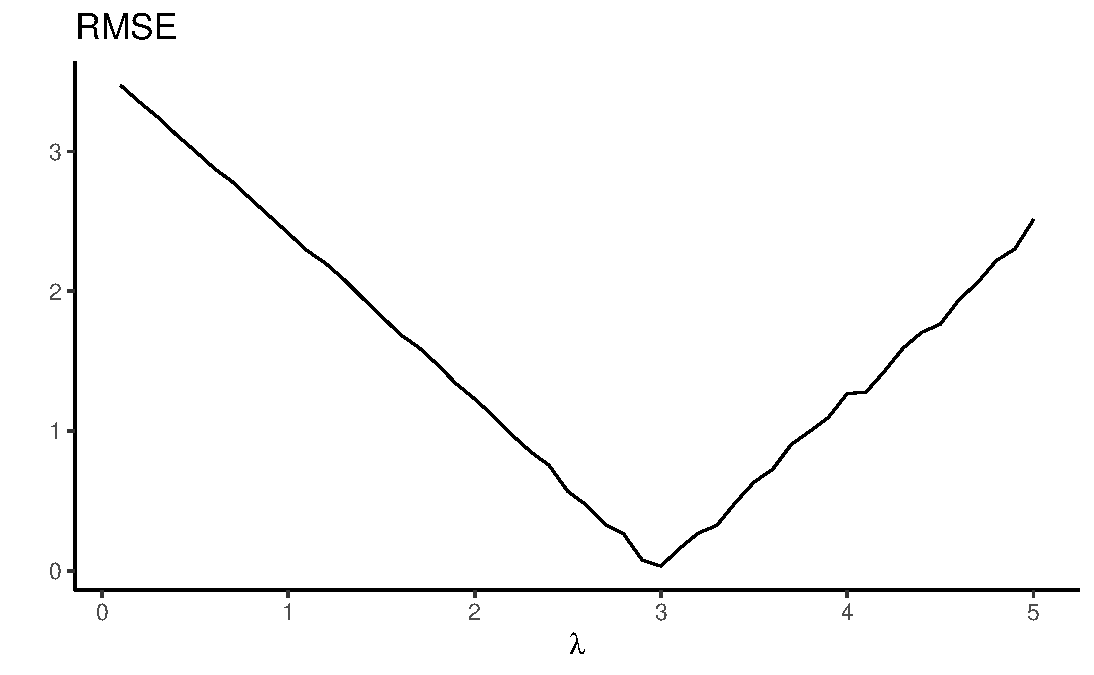
\includegraphics[width=0.4\textwidth]{../figures/lambda_pure_RMSE}
      \label{sub:lambda_pure_RMSE}
    }
    \subfloat[$\mu\mapsto d\left(p_{1:n},p_{1:n}^{\theta}\right)\Big\rvert_{\sigma =1, \lambda = 3}$]{
      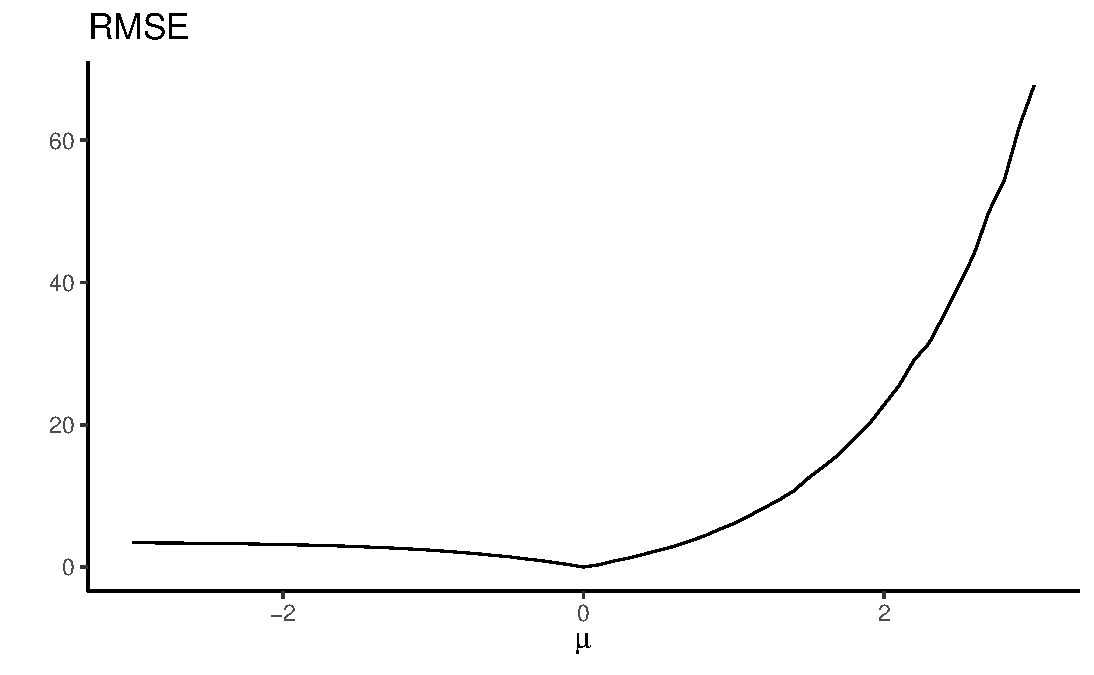
\includegraphics[width=0.4\textwidth]{../figures/mu_pure_RMSE}
      \label{sub:mu_pure_RMSE}
    }\\
    \subfloat[$\sigma\mapsto d\left(p_{1:n},p_{1:n}^{\theta}\right)\big\rvert_{\mu =0, \lambda = 3}$
    ]{
      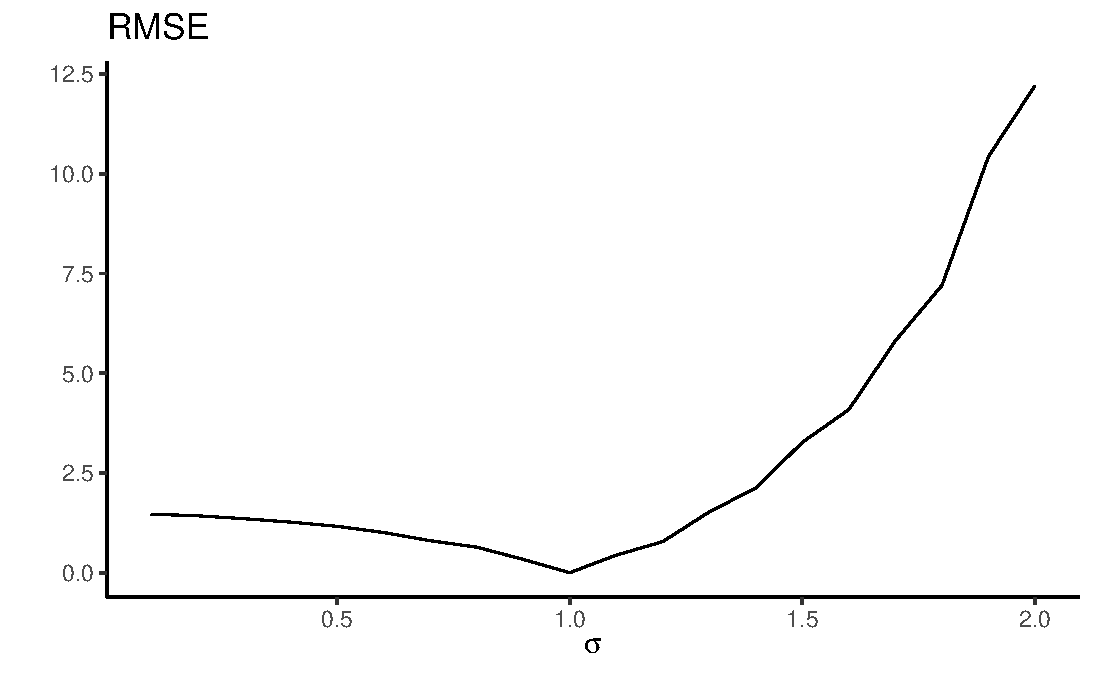
\includegraphics[width=0.4\textwidth]{../figures/sig_pure_RMSE}
      \label{sub:sig_pure_RMSE}
    }
    \caption{Plots of the RMSE when looking into each parameter separately.}
    \label{fig:rmse_pure_premium}
  \end{center}
\end{figure}

By taking the parameters separately, it looks like the model is identifiable. It does not mean that we can identify a unique parametrization if we do not fix two parameters out of three. We cannot use a grid search procedure to explore the three dimensional parameter space and so we use the optimization procedure described in Section 3.3 of our paper. The parameters of the algorithm are set as follows: 
$$
J = 500,\text{ }R= 500\text{, and } \epsilon_{\min} = 0.02.
$$
Recall that $J$ is the population size of the clouds of particles, $R$ is the number of Monte Carlo replications and $\epsilon_{\min}$ is a threshold for the tolerance level. The algorithm will stop if the tolerance threshold reaches $\epsilon_{\min}$. The prior distribution of the parameters are given by 
$$
\lambda \sim \UnifDist([0, 10]),\text{ }\mu\sim \UnifDist([-3, 3])\text{ and }\sigma\sim \UnifDist([0, 2]).
$$

\begin{figure}[!ht]
  \begin{center}
    \subfloat[Posterior distribution of $\lambda$]{
      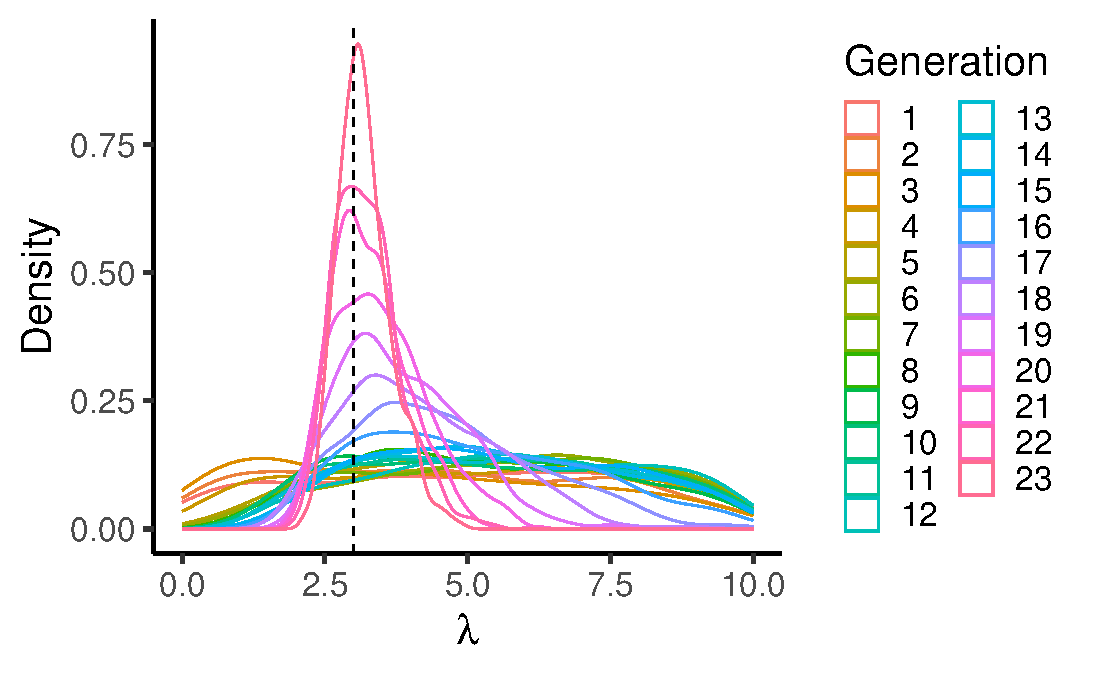
\includegraphics[width=0.4\textwidth]{../figures/posterior_lambda_supp_mat}
      \label{sub:posterior_lambda_supp_mat}
    }
    \subfloat[Posterior distribution of $\mu$]{
      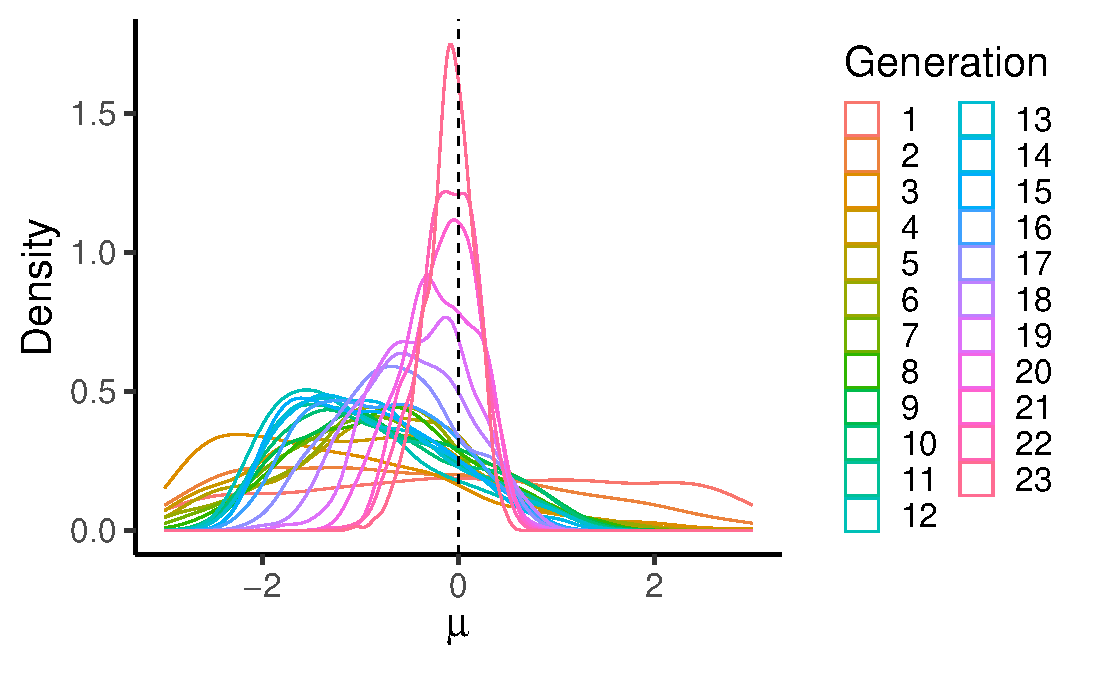
\includegraphics[width=0.4\textwidth]{../figures/posterior_mu_supp_mat}
      \label{sub:posterior_mu_supp_mat}
    }\\
    \subfloat[Posterior distribution of $\sigma$]{
      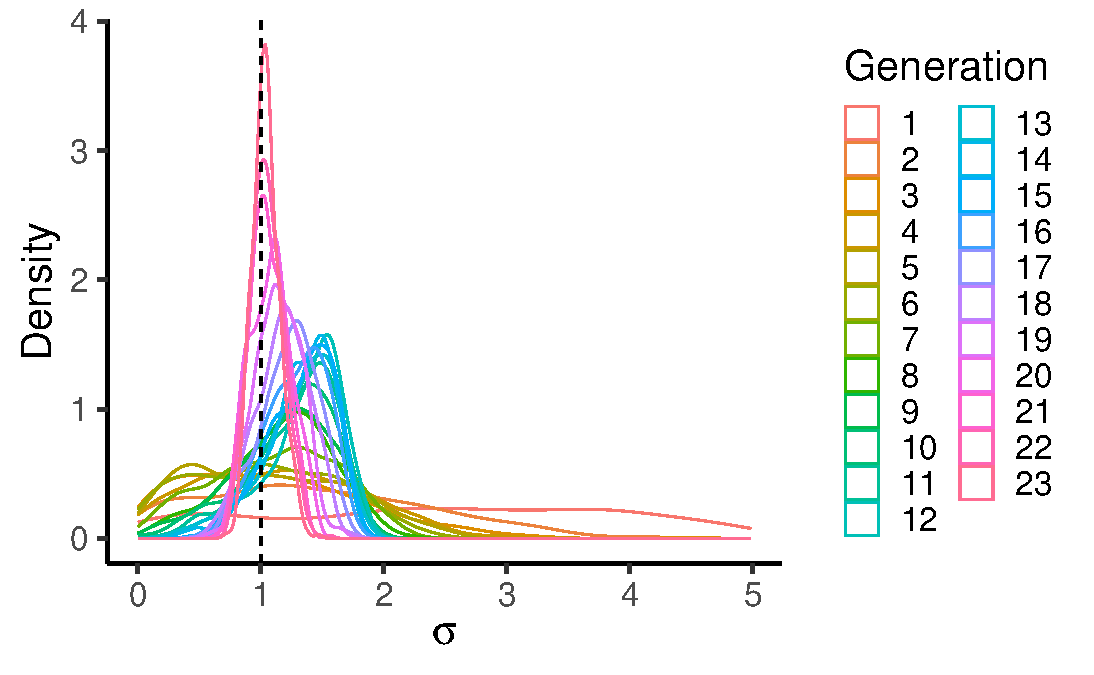
\includegraphics[width=0.4\textwidth]{../figures/posterior_sig_supp_mat}
      \label{sub:posterior_sig_supp_mat}
    }
    \caption{Posterior distributions of the parameters of the $\text{Pois}(\lambda)-\text{LogNormal}(\mu , \sigma)$ risk model.}
    \label{fig:posterior_pure_premium}
  \end{center}
\end{figure}

The choice of the level of $\epsilon_{\min} = 0.02$ follows from an estimation of the error on the RMSE resulkting from the use of a Monte Carlo approximation to calculate the pure premium. If we were able to compute exactly the pure premium then our algorithm should return some dirac distributions pointing to the true parameter value. The fact that we must use a Monte Carlo approximation justifies the use of an Approximate Bayesian Computation procedure as we encapsulate in the posterior distribution the uncertainty associated to the Monte Carlo error. Here we conclue that with these three pure premium allows us to identify the true parameters of the model. The situation is more difficult when we only have access to thecommercial premium as in the forthcoming section.
\section{Optimization problem 2}\label{sec:problem2}

As mentionned earlier, we do not have access to the pure premiums. Instead we have a collection of commercial rates $\Tilde{p}_{1:n} = \{\Tilde{p}_{1},\ldots, \Tilde{p}_{n}\}$ defined as
$$
\Tilde{p}_i = f_i(p_i) = f_i\left\{\mathbb{E}_{\theta_0}\left[g_{i}(X)\right]\right\},\text{ }i = 1,\ldots, n.
$$
It leads us to formulate the following optimization problem: 
\begin{pb}\label{pb:optimization_problem}
Denote by 
$$
p_i^\theta =\mathbb{E}_\theta\left[g_{i}(X)\right],\text{ for }i = 1,\ldots, n,
$$
the pure premium associated to a risk $X$ parametrized by $\theta\in \Theta\subset\mathbb{R}^d$. Further denote by $p^\theta_{1:n}$ and $\Tilde{p}_{1:n}$ the collections of pure and commercial premiums. \\

We wish to find $\theta\in \Theta\subset\mathbb{R}^d$ and $f:\mathbb{R}_+\mapsto \mathbb{R}_+$ to minimize \(d\left[\Tilde{p}_{1:n}, f(p_{i:n}^\theta)\right]\),

where the function $f$ is applied elementwise  on $p_{i:n}^\theta$ and $d(\cdot, \cdot)$ denotes a distance function over the observation space,
subject to 
\begin{equation}\label{eq:constraint1}
\Tilde{p}_i \geq p_i^\theta
\end{equation}
and 
\begin{equation}\label{eq:constraint2}
f(p_i^\theta) \geq p_i^\theta, 
\end{equation}
for $i = 1,\ldots, n$. 
\end{pb}

Our first task is to find a generic function $f$ to represent the safety loading functions $f_i$'s used by the competitors. For this, we use isotonic regression. It is a statistical technique used for fitting a non-decreasing function to a set of data points. The idea is that if two pure premium satisfy $p_i\leq p_j$ then the commercial premium should also verify $\Tilde{p}_i\leq \Tilde{p}_j$. Consider a collection of candidate pure premiums $p_{i:n}^\theta$, associated to a candidate risk parameter $\theta$. Our datapoints are therefore pairs of pure and commercial premiums $(p_i^\theta,\Tilde{p}_i)_{i=1,\ldots, n}$. Suppose the pure premium have been ordered such that $p_i^\theta\leq p_j^\theta$ for $i\leq j$, isotonic regression seeks a least square fit $\Tilde{p}^\theta_i$ for the $\Tilde{p}_i$'s such that $\Tilde{p}^\theta_i\leq \Tilde{p}^\theta_j$ for $p_i^\theta\leq p_j^\theta$. It reduces to find $\Tilde{p}^\theta_1,\ldots, \Tilde{p}^\theta_n$ that minimize
$$
\sum_{i=1}^nw_i^{\textsc{iso}}(\Tilde{p}^\theta_i- \Tilde{p}_i)^2\text{, subject to }\Tilde{p}_i^\theta\leq \Tilde{p}^\theta_j\text{ whenever }p_i^\theta\leq p_j^\theta,
$$
where $\left(w_i^{\textsc{iso}}\right)_{i = 1, \ldots, n}$ denotes the weights associated to each pair $(p_i^\theta,\Tilde{p}_i)_{i=1,\ldots, n}$. Since the $p_i^\theta$'s fall in a totally ordered space, a simple iterative procedure called the Pool Adjacent Violators Algorithm (PAVA) can be used. Here's a high-level overview of how it works:
\begin{enumerate}
\item Initialize the sequence of values to be the same as the data points $\Tilde{p}_i^\ast =\Tilde{p}_i$.

\item Iterate through the sequence and identify "violations," which occur when the current value is greater than the next value, that is 
$$
\Tilde{p}_i^\ast>\Tilde{p}_{i+1}^\ast\text{ for some }i=1,\ldots, n.
$$ 
When a violation is found, adjust the values in the associated segment of the sequence to be the average of the values,
$$
\Tilde{p}_i^\ast \leftarrow (\Tilde{p}_i^\ast + \Tilde{p}_{i+1}^\ast)/2,
$$ 
ensuring monotonicity.
\item Repeat Step 2 until no violations are left. 
\end{enumerate}
We use the \texttt{isoreg} function from $R$ to get the fitted values $\Tilde{p}^\theta_i,\text{ }i=1,\ldots, n$. To complete the isotonic regression task we shall find a function $f$ such that $f(p_i^\theta)=\Tilde{p}^\theta_i$. A common choice is a piece-wise constant function that interpolates the $\Tilde{p}^\theta_i$'s. We now turn to the definition of a distance. Our starting point to measure the discrepancy between observed and model-generated commercial rates is the root mean square error (RMSE) defined as
\begin{equation}\label{eq:sse_distance}
\text{RMSE}\left[\Tilde{p}_{1:n}, f(p^\theta_{i:n})\right] = \sqrt{\sum_{i=1}^nw^{\text{RMSE}}_i [\Tilde{p}_i - f(p_i^\theta)]^2},
\end{equation}
for a candidate risk parameter $\theta$ and an isotonic fit $f$. We seek 
$$
\theta^\ast = \underset{\theta\in \Theta}{\argmin}\,
\text{RMSE}\left[\Tilde{p}_{1:n}, f(p^\theta_{i:n})\right].
$$

The existence of such $\theta^\ast$ is guaranteed because $\theta\mapsto \text{RMSE}\left[\Tilde{p}_{1:n}, f(p^\theta_{i:n})\right]$ only takes a finite number of values. Indeed, to each $\theta \in \Theta$ is associated a unique permutation $s^\theta\in S_n$, where $S_n$ denotes the set of all the permutations of $\{1,\ldots, n\}$, such that 
$$
p^\theta_{s^\theta(1)}\leq\ldots\leq p^\theta_{s^\theta(n)}.
$$
This permutation $s^\theta$ defines a unique isotonic fit $f$ based on 
$$
\Tilde{p}^\theta_{s^\theta(1)}\leq\ldots\leq \Tilde{p}^\theta_{s^\theta(n)},
$$
leading to a given RMSE value $\text{RMSE}\left[\Tilde{p}_{1:n}, f(p^\theta_{i:n})\right]$. Concretely, for $\theta_1,\theta_2\in \Theta$, if it holds that $s^{\theta_1} = s^{\theta_2}$ then $\text{RMSE}\left[\Tilde{p}_{1:n}, f(p^{\theta_1}_{i:n})\right] = \text{RMSE}\left[\Tilde{p}_{1:n}, f(p^{\theta_2}_{i:n})\right]$. The application $\theta\mapsto s_n^\theta$ is surjective since $S_n^\Theta = \{s_n^\theta\text{ ; }\theta\in \Theta\}\}$  is finite.  The fact that $\Theta$ is a continuous space implies that $\theta^\ast$ cannot be unique. Our problem is an ill-posed inverse problem. Ill-posedness is usually dealt with by adding a regularization to the objective function that one wants to minimize. The ratio of \(p / \Tilde{p}\) corresponds to what practitioners would call the expected Loss Ratio (\(\text{LR}\)). Our solution is based on targeting a given loss ratio.  The loss ratio is a standard measure to assess the profitability of insurance lines of business. An insurance company that enters a new market is likely to have insights on the loss ratio relative to this market, for example by having informal discussions with reinsurers, brokers or competitors. These insights may translate into the definition of a lower and upper bound denoted by \(\text{LR}_{\text{low}}\) and \(\text{LR}_{\text{high}}\), respectively. We can then assume that the loss ratios \(\text{LR}_i = p_i / \Tilde{p}_i\), for \(i = 1, \ldots, n\), should fall in the range \([\text{LR}_{\text{low}}, \text{LR}_{\text{high}}]\), which we refer to as the loss ratio corridor. Assuming that \(\text{LR}_{\text{high}} < 1\), we may ensure both constraint \eqref{eq:constraint1} and \(\text{LR}_i \in [\text{LR}_{\text{low}}, \text{LR}_{\text{high}}]\) by adding to our distance \eqref{eq:sse_distance} two regularization terms defined as
\begin{equation*}\label{eq:LR_bounds1}
\text{Reg}_{\text{low}}\left(\Tilde{p}_{1:n}, p_{1:n}^\theta\right) = \sqrt{\sum_{i=1}^nw_i^{\text{RMSE}}\left(\Tilde{p}_i - p_i^\theta \cdot \text{LR}_{\text{low}}^{-1}\right)_+^2}, 
\end{equation*}
and 
\begin{equation*}\label{eq:LR_bounds2}
\text{Reg}_{\text{high}}\left(\Tilde{p}_{1:n}, p_{1:n}^\theta\right) = \sqrt{\sum_{i=1}^nw_i^{\text{RMSE}}\left(p_i^\theta \cdot \text{LR}_{\text{high}}^{-1} - \Tilde{p}_i\right)_+^2},
\end{equation*}
where \((x)_+ = \max(x,0)\) denotes the positive part of \(x\). The distance we consider within \cref{pb:optimization_problem} is now given by 
\[
d\left[\Tilde{p}_{1:n}, f(p_{1:n}^\theta)\right] = \text{RMSE}\left[\Tilde{p}_{1:n}, f(p_{1:n}^\theta)\right] + \text{Reg}_{\text{low}}\left(\Tilde{p}_{1:n}, p_{1:n}^\theta\right) + \text{Reg}_{\text{high}}\left(\Tilde{p}_{1:n}, p_{1:n}^\theta\right).
\]
We take again our three insurance coverages $g_1, g_2$ and $g_3$ and we distinguish two safety loading situations. The well-specified case in \cref{ssec:well_specfifed_safety_loading} and the miss-specified on in \cref{ssec:miss_specfifed_safety_loading}
\subsection{Well-specfifed safety loading}\label{ssec:well_specfifed_safety_loading}
Consider the following loading functions
$$
f_1(x) = 1.38\cdot x\text{, }f_2(x) = 1.1\cdot x \text{, and } f_3(x) = 1.4\cdot x. 
$$
The isotonic model is well specified in this case because the pure and commercial premium are ordered in the same way. In that case the isotonic regression exactly interpolates the datapoints as shown on \cref{fig:pp_cp_well_specified}.

\begin{figure}[!ht]
  \begin{center}
  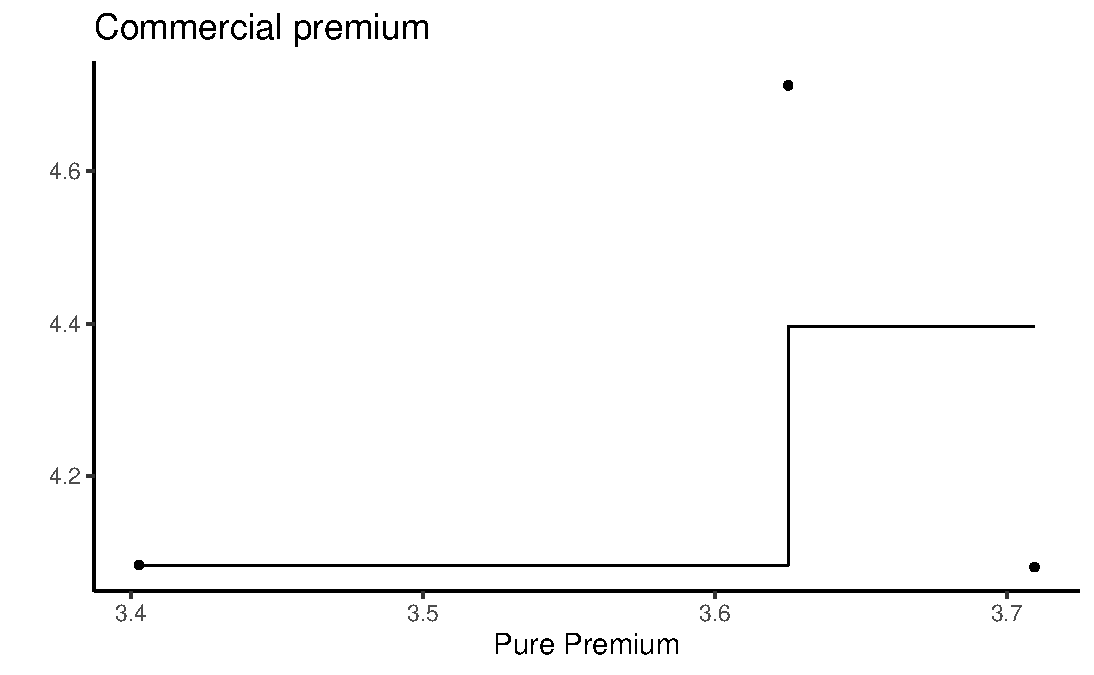
\includegraphics[width=0.7\linewidth]{../figures/pp_cp_well_specified}
    \caption{Intermediate posterior distributions for $\lambda$ and $\sigma$.}
    \label{fig:pp_cp_well_specified}
  \end{center}
\end{figure}

\cref{sub:sig_pure_RMSE} shows the plot of the $\sigma\mapsto d\left(p_{1:n},p_{1:n}^{\theta}\right)\Big\rvert_{\lambda =3, \mu =0}$ when $f$ is isotonic (\cref{sub:rmse_sigma_iso}) and when $f$ is linear (\cref{sub:rmse_sigma_linear}).

\begin{figure}[!ht]
  \begin{center}
    \subfloat[$f$ is isotonic]{
      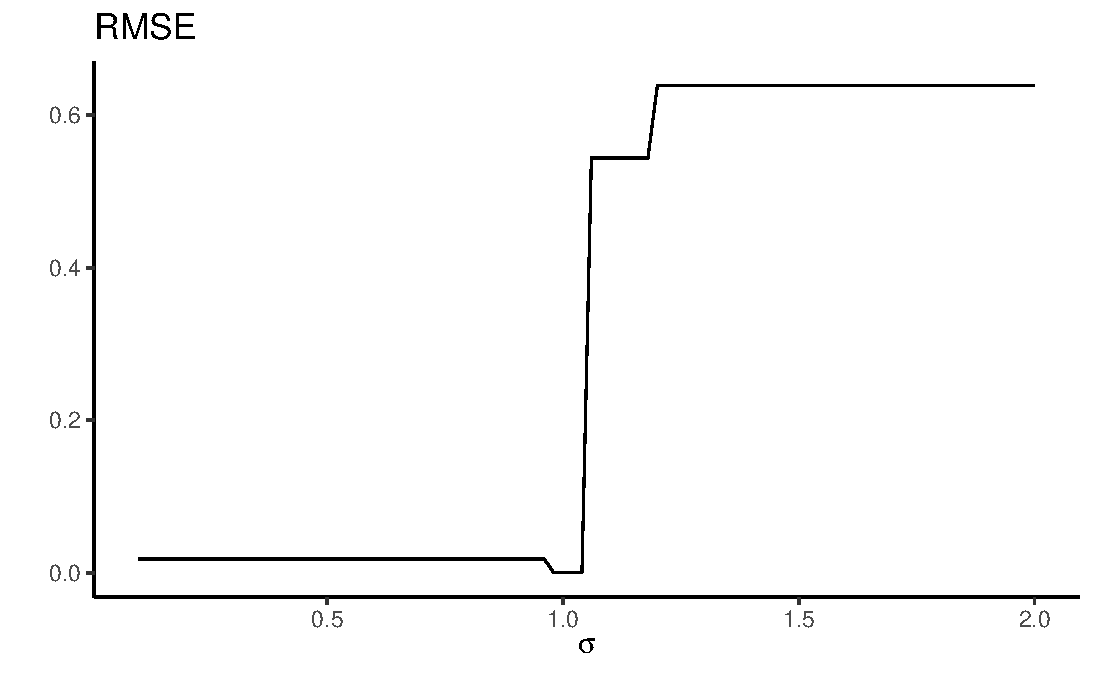
\includegraphics[width=0.4\textwidth]{../figures/rmse_sigma_iso}
      \label{sub:rmse_sigma_iso}
    }
    \subfloat[$f$ is linear]{
      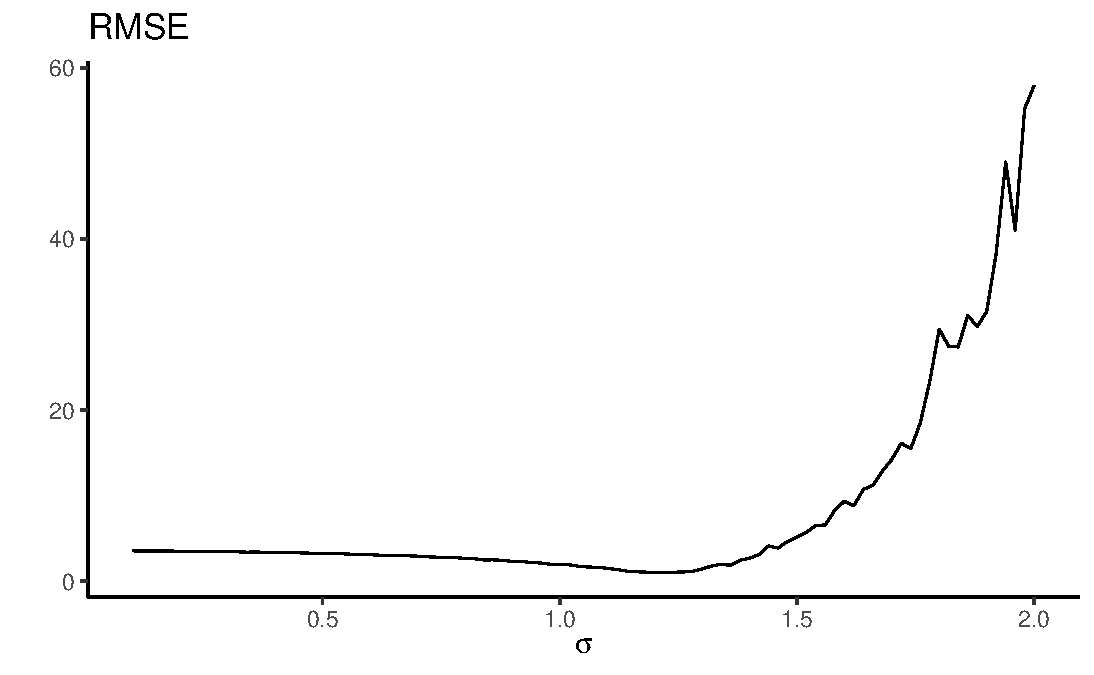
\includegraphics[width=0.4\textwidth]{../figures/rmse_sigma_linear}
      \label{sub:rmse_sigma_linear}
    }
    \caption{$\sigma\mapsto d\left(p_{1:n},p_{1:n}^{\theta}\right)\Big\rvert_{\mu =0, \sigma = 1}$.}
    \label{fig:rmse_sigma_iso_linear}
  \end{center}
\end{figure}

Note that in this example we do not cancrel the regularization terms. When $f$ is isotonic, the values of $\sigma$ for which the RMSE is null are associated to the same ordering of the pure premium than that of the true parameter $\sigma=1$, see \cref{sub:rmse_sigma_iso}. Several values of $\sigma$ are therefore optimal including the true one. On the other hand, when $f$ is linear, the RMSE is minimal for the parameter value that manage to align the commercial premium. It looks like one value of $\sigma$ however it is far from the true value, see \cref{sub:rmse_sigma_linear}. When looking at \cref{sub:rmse_sigma_iso}, one might expect that by running our ABC algorithm we shall get a uniform distribution as posterior distribution. We set the parameters of the algorithm as 
$$
J = 2000\text{, }R= 500\text{, and }\epsilon_{\min} =10^-8.
$$
We set a prior distribution on $\sigma$ as $\sigma\sim\UnifDist([0, 2])$. The tolerance level is very low as we are after the values of sigma that yields the right ordering associated to a nearly null RMSE. The posterior distribution is provided on \cref{fig:posterior_sig_iso_supp_mat}.

\begin{figure}[!ht]
  \begin{center}
  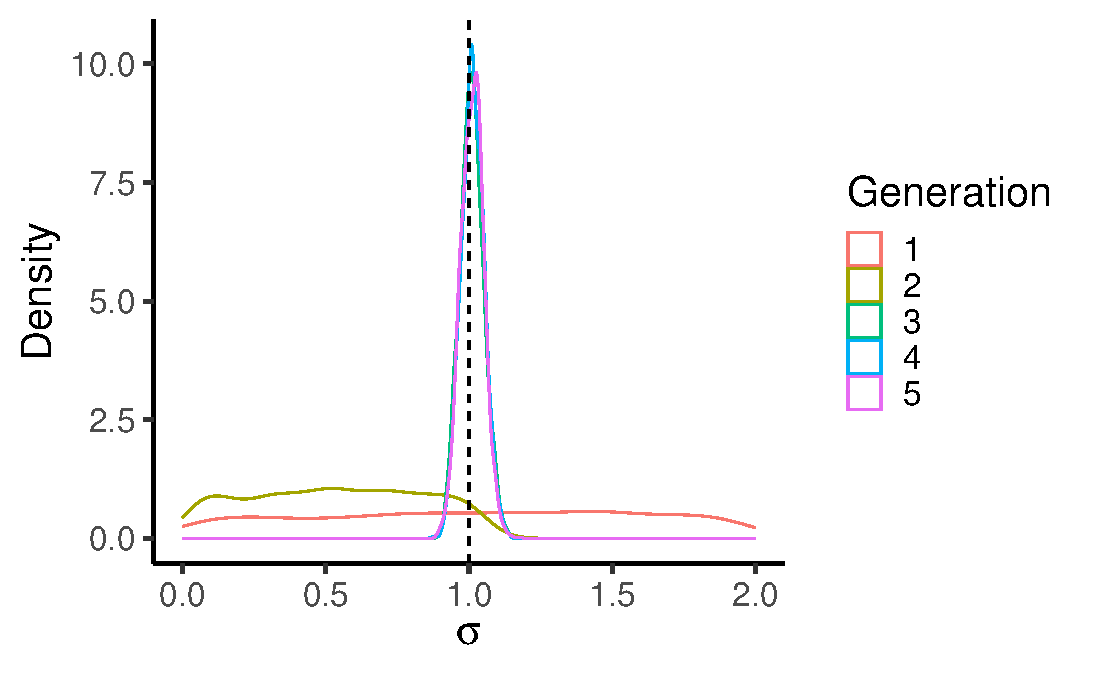
\includegraphics[width=0.7\linewidth]{../figures/posterior_sig_iso_supp_mat}
    \caption{Intermediate posterior distributions for $\sigma$.}
    \label{fig:posterior_sig_iso_supp_mat}
  \end{center}
\end{figure}

It turns out that the posterior distribution is not all that uniform, this is explained by the Monte Carlo approximation we use which might change the pure premium ordering when getting close to the edge of the range of admissible $\sigma$ values. The posterior distribution displayed on \cref{fig:posterior_sig_iso_supp_mat} could look good enough to the naive eye and one could argue that regularization is not required here. When looking for $\lambda$, $\mu$ and $\sigma$ at the same time the parameters can offset each other and the right ordering of the pure premium does not allow us to extract relevant information. We run our ABC algorithm with the following settings 
$$
J = 500\text{, }R= 500\text{, and }\epsilon_{\min} =10^-8.
$$
The prior distributions on the model parameters are as follows: 
$$
\lambda \sim \UnifDist([0, 10]),\text{ }\mu\sim \UnifDist([-3, 3])\text{ and }\sigma\sim \UnifDist([0, 2]).
$$
The posterior distribution are provided on \cref{sub:sig_pure_RMSE}.

\begin{figure}[!ht]
  \begin{center}
    \subfloat[Posterior distribution of $\lambda$]{
      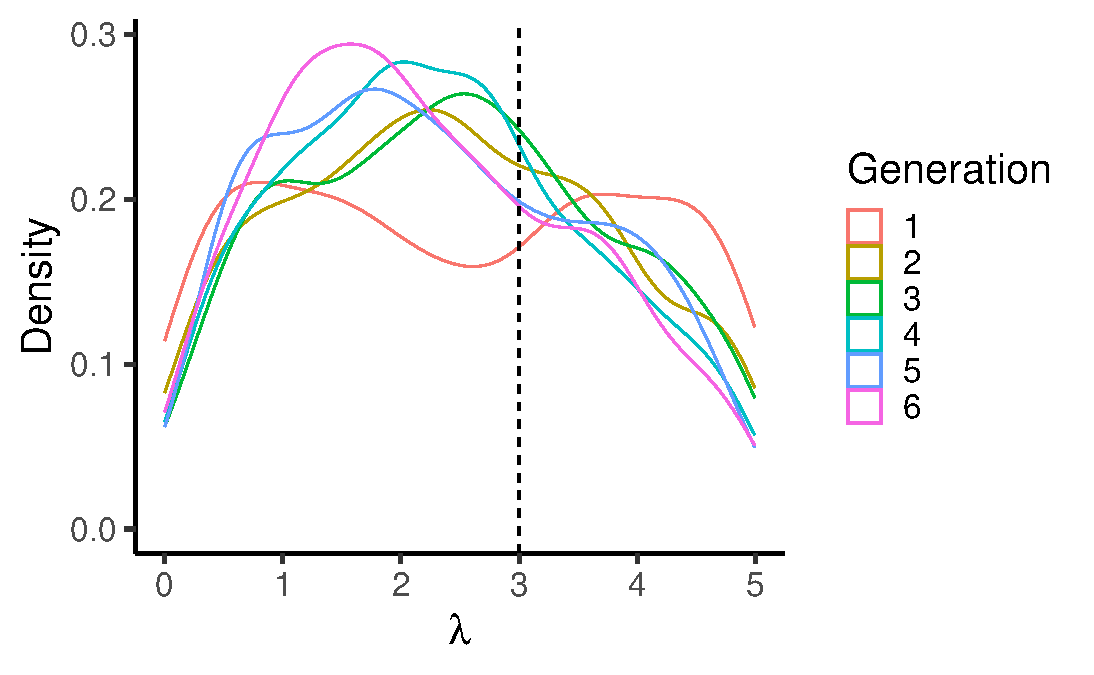
\includegraphics[width=0.4\textwidth]{../figures/posterior_lambda_wo_reg_supp_mat}
      \label{sub:posterior_lambda_wo_reg_supp_mat}
    }
    \subfloat[Posterior distribution of $\mu$]{
      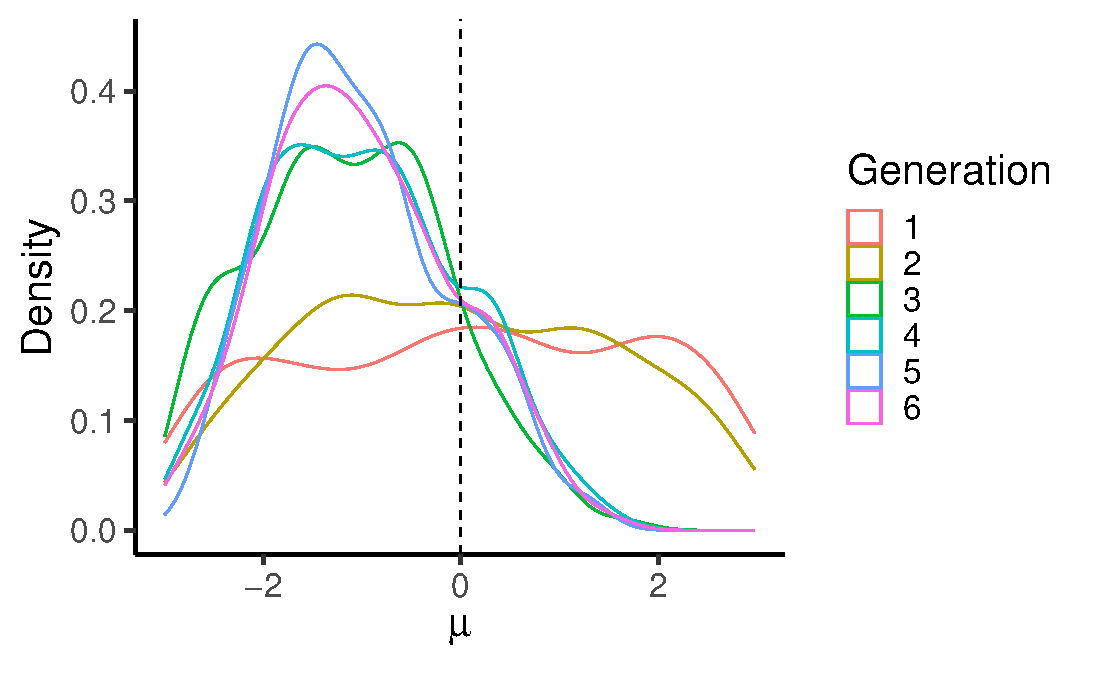
\includegraphics[width=0.4\textwidth]{../figures/posterior_mu_wo_reg_supp_mat}
      \label{sub:posterior_mu_wo_reg_supp_mat}
    }\\
    \subfloat[Posterior distribution of $\sigma$]{
      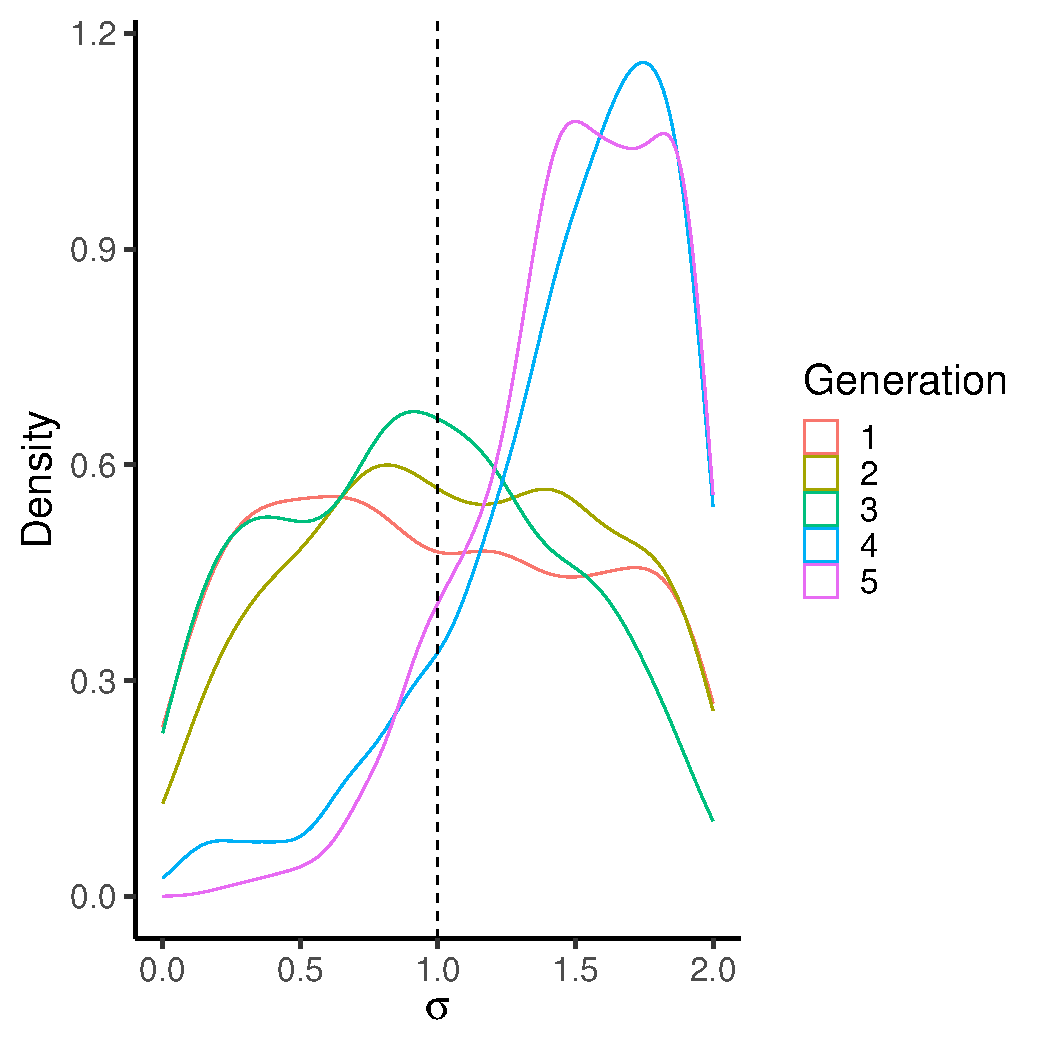
\includegraphics[width=0.4\textwidth]{../figures/posterior_sig_wo_reg_supp_mat}
      \label{sub:posterior_sig_wo_reg_supp_mat}
    }
    \caption{Posterior distributions of the parameters of the $\text{Pois}(\lambda)-\text{LogNormal}(\mu , \sigma)$ risk model.}
    \label{fig:posterior_commercial_premium_wo_reg}
  \end{center}
\end{figure}

Too many combination of parameters yield the right ordering. Only regularization can help us in discriminating the irrelvant portions of the parameter space.

\subsection{Misspecified safety loading} \label{ssec:miss_specfifed_safety_loading}

\bibliographystyle{plainnat}
\bibliography{abc_no_data}


\end{document}